\chapter{Literature Review}
  \section{Space Exploration and NASA's Journey to Mars}
    \subsection{A Brief History}
      The human race possesses a trait that proposedly sets us apart from the majority of life forms around us; the powerful will to explore what is unknown. It is the curiosity and the thrill to push past the boundaries of what is thought to be possible, perhaps felt stronger by some, that forms the basis of many scientific endeavours relating to facts of life and existence around and outside of the immediate environment in which we live.
      
      A prime example of such a drive to explore is in the research and exploration of outer space, which, from a technological perspective, transitioned from astronomer's dream to scientist's and engineer's reality during the Cold War. Although space exploration as we know it today is motivated by human curiosity, it was during this period of political tension that significant breakthroughs in spacecraft and rocket propulsion technology were brought about. This period is referred to as the ``Space Race'' and stemmed from research and development of nuclear weaponry during World War II \cite[p. 147]{cornwell2003hitler}. The race began with the attempted launches of artificially made satellites \cite[pp. 3-5]{schefter1999the} and within the 40 years following the success of the USSR's \textit{Sputnik I} in 1957, the first object to be put into orbit by man, space technology progressed from early manned flights beginning in 1961\footnote{First human in space, Soviet launched} through the \textit{Apollo 11} lunar flight to having flown by of the majority of the planets in our solar system.
      
      By 1981, the launch of \textit{Columbia} \cite{williamharwood2009}, a space shuttle designed to be used for more than one flight, marked the beginning of reusable space technologies answering to the problem of cost and with the forethought of future increase in space flight frequency and demand. Today, the efforts to lower the cost of space travel and the attempt to bring space exploration into the private sectors to make these opportunities more realisable by the public are evident in Elon Musk's SpaceX development of the Falcon 9, a reusable rocket that returns and lands safely back on the surface of Earth \cite{spacex_popularmechanics}.
      
      The National Aeronautics and Space Administration (NASA) of the United States has been and still is responsible for a large chunk of mankind's search among the stars and, with respect to research and exploration, has made great efforts to better understand the planet that we live on in conjunction with the immediate spacial environment around Earth, the solar system and the planets within, and that which lies in deep space. After the Apollo lunar missions, efforts by NASA to explore involved one of the first space stations, the \textit{Skylab}, which suffered technical difficulties originating from launch but proved the ability to conduct research in space as well as allow astronauts to perform repairs and maintenance to artificial bodies in that environment \cite{compton1983living}. \textit{Skylab} was followed by the International Space Station (ISS), intended to be a more sustainable microgravity environment in which to conduct research that might require such conditions. Research of this type include a very broad range of investigations from the effects of near-weightlessness on plants and animals through to growth of human-like tissues and protein crystallisation \cite{nasaresearch}. An area of research that specifically relates to this project is in the development of technology to allow for longer, cheaper and faster flights in space, both in spacecraft materials and systems and in astronaut health and performance. This is closely coupled with the search by entities around the world for other forms of life outside of Earth's atmosphere fuelled by the prospect of finding environmental architectures similar to ours. One of NASA's goals outlined in \cite{nasa2010act} is to send humans to Mars and this has lead to enormous amounts of research, promising engineering and technological successes that will ultimately allow humankind to extend civilisation across more than one planet.
    
    \subsection{Mars} 
      NASA has identified that Mars is a planet with greater similarity in formation and conditions in its history and as a result has been a target of exploration for more than 40 years. This has involved multiple flybys and orbits starting from 1962 through to the first lander, the \textit{Viking 1}, to touch down on the surface of the planet in 1975 \cite{marsprogram2008}. NASA's Jet Propulsion Laboratory (JPL) landed the spacecraft, named \textit{Pathfinder}, that contained the first successful rover vehicle, the \textit{Sojourner}, in 1997 \cite{pathfindersojournerjpl}. The purpose of this mission was to prove the possibility of cheaper spacecraft development and the transport of scientific equipment to the planet as well as taking photographs of the red surface, from the surface. 
    
    
    % TODO: NASA and Mars
    % Something about why we need rovers and what was NASA's goal etc
    
  \section{The Mars Science Laboratory and Curiosity}
    \subsection{Overview}
      The Mars Science Laboratory (MSL) is a mission that was launched by NASA to further explore the surface of Mars, one of many orbiter, lander and rover type missions as part of the Jet Propulsion Laboratory's (JPL\footnote{Jet Propulsion Laboratory of California Institute of Technology}) Mars Exploration Program (MEP). The program is structured to work towards a set of goals to ultimately understand and determine the potential for life on Mars \cite{meptheme} by observation of the current climate and geology. The MSL is the latest mission in operation as part of MEP and was intended to span roughly one Martian year after touchdown on Mars. However, it has continued to operate for more than double that amount of time. 
      
      \begin{figure}[ht]
        \centering
        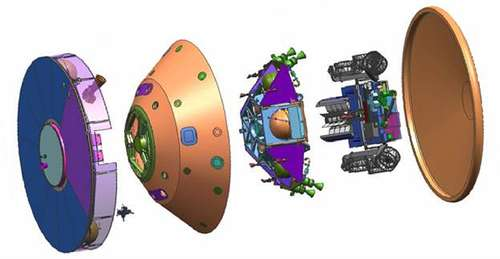
\includegraphics[width=0.7\textwidth]{figures/mslSpacecraftExplodedView.jpg}
        \label{fig:mslSpacecraftExplodedView}
        \caption{An exploded 3D model of the Mars Science Laboratory spacecraft including the cruise stage (far left) and heat shield (far right) \cite{fig:mslSpacecraftExplodedView_cite}}
      \end{figure}
      
      
      MSL was launched from Cape Canaveral Space Station, Launch Complex 41, atop an Atlas V vehicle, a two stage rocket \cite{harwood2014sfn}. The mission required the launch vehicle to insert the five-piece MSL spacecraft into a transfer orbit in a process known as a Trans-Mars Injection (TMI) allowing the spacecraft to arrive at Mars after a 566 million kilometre trip that lasted 256 days. Figure~\ref{fig:mslSpacecraftExplodedView} shows a 3D render of the components of the spacecraft that made the trip. Four trajectory correction manoeuvres were made during the flight to result in a landing near ``Mount Sharp'' in Gale Crater, deemed the most accurate landing on Mars of any other spacecraft \cite{martinmur}.
      
      % TODO: Launch site choice
    
    \subsection{Primary Mission Goals and Objectives}
      Touching down on the surface of Mars, the MSL had primary objectives tailored to contribute to the four goals as outlined in the MEP. The objectives were carried out by the MSL's flagship component, the Curiosity rover, and consisted of a wide range of biological and geological observations such as to determine the chemical building blocks that exist on the surface including organic carbon compounds, prospective historical biological activity, atmospheric processes of evolution, surface radiation and state and distribution of water \cite{mslobjectivesjpl}.
      
      Apart from the primary objectives, the MSL mission pushes further the boundaries of space exploration in that it proved the ability to land heavier vehicles at incredibly precise landing accuracy as well as the achievement of wider surface coverage to collect and observe more diverse samples of the surface of Mars.
              
    \subsection{Technical Breakdown of the Curiosity Rover}
      23\% of the MSL spacecraft's total mass of 3.893 metric tonnes was thanks to the missions vehicle, \textit{Curiosity} . The six wheeled, instrument bearing rover features much improved hardware over previous vehicles along with a multiple systems of instruments to enable the carrying out of the mission objectives. The mechanical and technological specifications are broken down in the sections to follow.
      
      \subsubsection{Mechanical Structure}
      
      \subsubsection{Rover Compute Element}
      
      \subsubsection{Manoeuvrability}
      
      \subsubsection{Instrumentation}
      
      \subsubsection{Communication}
      
      

  \section{Space Education and Outreach}
  
  \section{Web Technologies for Modern Outreach}
  
  \section{Additive Prototyping and Manufacturing Techniques}